%% LyX 2.3.6.1 created this file.  For more info, see http://www.lyx.org/.
%% Do not edit unless you really know what you are doing.
\documentclass[10pt,twoside,english]{article}
\usepackage{lmodern}
\usepackage[latin9]{inputenc}
\usepackage[a4paper]{geometry}
\geometry{verbose,tmargin=2cm,bmargin=2cm,lmargin=2cm,rmargin=2cm,headheight=1cm,headsep=1cm,footskip=1cm}
\usepackage{fancyhdr}
\pagestyle{fancy}
\usepackage{color}
\usepackage{babel}
\usepackage{array}
\usepackage{booktabs}
\usepackage{calc}
\usepackage{units}
\usepackage{textcomp}
\usepackage{amsmath}
\usepackage{amssymb}
\usepackage{graphicx}
\usepackage[unicode=true,
 bookmarks=true,bookmarksnumbered=false,bookmarksopen=false,
 breaklinks=false,pdfborder={0 0 1},backref=false,colorlinks=true]
 {hyperref}
\hypersetup{pdftitle={DassFlow 2 : User and Developer Guide},
 pdfauthor={Frederic Couderc}}

\makeatletter

%%%%%%%%%%%%%%%%%%%%%%%%%%%%%% LyX specific LaTeX commands.
\DeclareFontEncoding{LGR}{}{}
\DeclareRobustCommand{\greektext}{%
  \fontencoding{LGR}\selectfont\def\encodingdefault{LGR}}
\DeclareRobustCommand{\textgreek}[1]{\leavevmode{\greektext #1}}
\ProvideTextCommand{\~}{LGR}[1]{\char126#1}

%% Because html converters don't know tabularnewline
\providecommand{\tabularnewline}{\\}
%% A simple dot to overcome graphicx limitations
\newcommand{\lyxdot}{.}


%%%%%%%%%%%%%%%%%%%%%%%%%%%%%% User specified LaTeX commands.
\usepackage{fancyhdr}
\usepackage{lastpage}
\usepackage{color}

\usepackage[affil-it]{authblk}

%\usepackage{indentfirst}

\author[1]{Contributors: see DassFlow webpage}

\affil[1]{Institut de Math�mathiques de Toulouse / INSA / CNRS / INRAe / ICUBE Strasbourg}


\renewcommand\Authands{ and }

\newcommand{\version}{v3.0}
\newcommand{\DassFlow}{\textsc{DassFlow}}

\newcommand{\bin}{\texttt{\textbf{/bin}}}
\newcommand{\cpp}{\texttt{\textbf{/cpp}}}
\newcommand{\doc}{\texttt{\textbf{/doc}}}
\newcommand{\code}{\texttt{\textbf{/code}}}
\newcommand{\libs}{\texttt{\textbf{/libs}}}
\newcommand{\obj}{\texttt{\textbf{/obj}}}
\newcommand{\cases}{\texttt{\textbf{/cases}}}
\newcommand{\souk}{\texttt{\textbf{/souk}}}
\newcommand{\src}{\texttt{\textbf{/src}}}
\newcommand{\tap}{\texttt{\textbf{/tap}}}
\newcommand{\tools}{\texttt{\textbf{/tools}}}

\newcommand{\binres}{\texttt{\textbf{/bin/res}}}
\newcommand{\binmsh}{\texttt{\textbf{/bin/msh}}}
\newcommand{\binobs}{\texttt{\textbf{/bin/obs}}}
\newcommand{\bingrad}{\texttt{\textbf{/bin/grad}}}
\newcommand{\binmin}{\texttt{\textbf{/bin/min}}}

\newcommand{\make}{\texttt{\textbf{Makefile}}}
\newcommand{\exe}{\texttt{\textbf{exe}}}

\newcommand{\inp}{\texttt{\textbf{input.txt}}}
\newcommand{\usr}{\texttt{\textbf{m\_user\_data.f90}}}
\newcommand{\tst}{\texttt{\textbf{m\_user\_test.f90}}}
\newcommand{\bc}{\texttt{\textbf{bc.txt}}}
\newcommand{\obs}{\texttt{\textbf{obs.txt}}}
\newcommand{\paramObs}{\texttt{\textbf{param\_obs.txt}}}
\newcommand{\hydro}{\texttt{\textbf{hydrograph.txt}}}
\newcommand{\rat}{\texttt{\textbf{ratcurve.txt}}}
\newcommand{\landuse}{\texttt{\textbf{land\_use.txt}}}

\newcommand{\warm}{\includegraphics[scale=0.25]{figs/Symbols-Critical-icon}}

\lhead{\DassFlow{} \version{} - User and Developer Guide}
\rhead{University of Toulouse - INSA/University of Strasbourg/INRAE/CNES/CNRS}
\cfoot{\thepage/\pageref{LastPage}}
\pagestyle{fancy}

\definecolor{mygreen}{rgb}{0,0.6,0}
\definecolor{mygray}{rgb}{0.5,0.5,0.5}
\definecolor{mymauve}{rgb}{0.58,0,0.82}

\lightrulewidth=.04em
\heavyrulewidth=.12em

\AtBeginDocument{
  \def\labelitemii{\(\triangleright\)}
  \def\labelitemiii{\normalfont\bfseries{--}}
  \def\labelitemiv{\(\ast\)}
}

\makeatother

\begin{document}
\title{Equations and Numerical Schemes coded in DassFlow2D}
\date{March 2022}

\maketitle
\tableofcontents{}

\clearpage{}

\section{Mathematical models \& data assimilation features}

DassFlow 2D is an open computational software designed to shallow
free surface flows with features of Variational Data Assimilation.
The dynamics flow model can be coupled with a hydrology model, therefore
providing a complete hydraulic-hydrology model.

The computational kernel is coded in Fortran 2003 / MPI. It is wrapped
in Python. \\
In the latest version, the following physical models are available:
the 2D SW equations in variables $(h,q_{x},q_{y})$, its version for
Herschel-Bulkley rheology (non Newtonian fluids, power-law rheology
with threshold) and the GR4H rainfall-rainoff model. 

Note that a 1D version of SW system in variables $(S,Q)$ (Saint-Venant's
equations) is available but in another DassFlow version (please consult
DassFlow webpage for details). 

\subsection{The 2D SW equations for Newtonian fluids}

Let us denote by $h$ the water depth (m), by $\mathbf{q}$ the discharge
($m^{3}/s$), $\mathbf{q}=h\mathbf{u}$, $\mathbf{u}=(u,v)^{T}$ the
depth-averaged velocity ($m/s$). 

On a computational domain $\Omega\in\mathbb{\mathbb{\mathbb{R}}}^{2}$
and for a time interval $\left[0,T\right]$, the equations numerically
solved are:

\begin{equation}
\left\{ \begin{array}{lclcc}
\partial_{t}h+div(\mathbf{q}) & = & 0 & \textrm{in} & \text{\textgreek{W}}\times]0,T]\\
\\
\partial_{t}\mathbf{q}+div\left(\dfrac{\mathbf{q}\otimes\mathbf{q}}{h}+g\dfrac{h^{2}}{2}Id\right) & +gh\mathbf{\nabla}z_{b} & =-g\dfrac{n^{2}\left\Vert \mathbf{q}\right\Vert }{h^{7/3}}\mathbf{q} & \textrm{in} & \text{\textgreek{W}}\times]0,T]
\end{array}\right.\label{eq:sw}
\end{equation}

where $g$ is the magnitude of the gravity, $z_{b}$ the bed elevation
and $n$ the Manning-Strickler roughness coefficient.\\
It is accompanied by initial and all usual boundary conditions necessary
for real-world applications.

In the sequel we denote by: $\mathbf{U}=\left(h,\boldsymbol{q}\right)=\left(h,h\boldsymbol{u}\right)=(h,q_{x},q_{y})$. 

\subsection{The 2D SW equations for Non-Newtonian fluids (Herschel-Bulkley rheology)}

For non-Newtonian flows, the SW equations with Herschel-Bulkley rheology
writes:

\begin{equation}
\left\{ \begin{array}{lclcc}
\partial_{t}h+div(\mathbf{q}) & = & 0 & \textrm{in} & \text{\textgreek{W}}\times]0,T]\\
\\
\partial_{t}\mathbf{q}+div\left(\dfrac{\mathbf{q}\otimes\mathbf{q}}{h}+\frac{1}{2}gh^{2}\textrm{cos}\theta\boldsymbol{I}+\xi h^{2m+3}\right) & = & -gh\left(\textrm{cos}\theta\nabla z_{b}-S_{\ensuremath{\theta}}\right)-\frac{1}{\rho}K\boldsymbol{\tau}_{b} & \textrm{in} & \text{\textgreek{W}}\times]0,T]
\end{array}\right.\label{eq:hb}
\end{equation}

where;\\
 $\xi=\left[\begin{aligned}\frac{1}{(2m+3)(m+2)^{2}}\left[\frac{\rho g}{K}S_{\ensuremath{\theta}}\right]^{2m}\end{aligned}
\right]$ and $S_{\ensuremath{\theta}}=\begin{cases}
\textrm{sin}\theta & \textrm{for flows with low viscosity }\\
\textrm{sin}\theta-\textrm{cos}\theta\nabla H & \textrm{for flows with relatively high viscosity}
\end{cases}$ \\
$K\boldsymbol{\tau}_{b}=\left[\begin{aligned}\tau_{c}+K\left[\frac{\boldsymbol{q}}{\left(h-\frac{\tau_{c}}{\rho gS_{\ensuremath{\theta}}}\right)\left(\frac{1}{m+1}h-\frac{1}{(m+1)(m+2)}\left[h-\frac{\tau_{c}}{\rho gS_{\ensuremath{\theta}}}\right]\right)+\left(\frac{\rho gS_{\ensuremath{\theta}}}{\rho gS_{\ensuremath{\theta}}h-\tau_{c}}\right)^{m}\left(\frac{z_{b}^{m+2}}{(m+1)(m+2)}+Ch^{m+1}\right)}\right]^{\frac{1}{m}}\end{aligned}
\right]$\\
with;\\
$\tau_{c}=\rho gS_{\ensuremath{\theta}}h_{p}(z,t)$, $h_{p}(z,t)=h(z,t)-h_{c}(z,t)$
and $m=\frac{1}{n}$ \\
where $n$ denotes the power-law index, $H$ the fluid elevation,
$\tau_{b}$ the\textbf{ }basal shear stress, $K(T)$ the consistency
index which is temperature-dependent, $\tau_{c}$ the yield stress
, $h_{c}$ the thickness of the sheared zone , $h_{p}$ the plug thickness,
and $C$ the basal slip coefficient. 

Similarly, the usual initial and boundary conditions are imposed.

\subsection{The bucket-type rainfall-runoff model}

The GR4H model (\cite{mathevet2005quels}) is a lumped continuous
model that runs at the hourly time step. It is based on the GR4J model
formulation of \cite{perrin2003improvement} and uses a robust and
parsimonious production function proposed in (\cite{michel1989modele}).
It is a well-established, parsimonious and robust model and its state-space
version (\cite{santos2018continuous}) is based on Ordinary Differential
Equations (ODEs) hence differentiable. This property is a necessary
condition to generate an adjoint code.

Several GR models exist, featuring varying amounts of parameters,
stores and time steps (see \cite{perrin2007modeles}). The ``state-space''
version of the GR4H model is described by the following set of ODEs
equations:

\begin{equation}
\frac{\mathrm{d}\boldsymbol{h}}{\mathrm{dt}}=\begin{cases}
\dot{h_{p}} & =P_{s}-E_{s}-P_{erc}\\
\dot{h}_{1} & =P_{r}-Q_{Sh,1}\\
\dot{h}_{2} & =Q_{Sh,1}-Q_{Sh,2}\\
... & ...\\
\dot{h}_{nres} & =Q_{Sh,nres-1}-Q_{Sh,nres}\\
\dot{h_{r}} & =Q_{9}+F-Q_{r}
\end{cases}\label{eq:GR4state-space}
\end{equation}

It consists in a production store $S$, a routing store $R$ and a
series of 11 Nash cascade stores $S_{h,i},\,\forall i\in\left[1..11\right]$.
The internal model variables are the 13 store levels. Four parameters
$\left(x_{1},\,x_{2},\,x_{3},\,x_{4}\right)$ rule the draining of
the production store, of the routing store, of the 11 identical cascading
stores and the non-conservative exchange law. Initial store states
are given using a 1 year warm-up period. 

They involve the following fluxes:

\begin{equation}
\begin{cases}
E_{s}= & E\left(\frac{2h_{S}}{c_{1}}-\left(\frac{h_{p}}{c_{1}}\right)^{\alpha}\right)\\
P_{S}= & P\left(1-\left(\frac{h_{p}}{c_{1}}\right)^{\alpha}\right)\\
P_{erc}= & \left(\frac{\nu}{c_{1}}\right)^{\beta-1}\frac{1}{\beta-1}\left(h_{p}^{+}\right)^{\beta}\\
P_{R}= & P\left(\frac{h_{p}}{c_{1}}\right)^{\alpha}+\left(\frac{\nu}{c_{1}}\right)^{\beta-1}\frac{1}{\beta-1}\left(h_{p}^{+}\right)^{\beta}\\
Q_{N1}= & \frac{n_{res}-1}{c_{4}}h_{1}^{+}\\
... & ...\\
Q_{N11}= & \frac{n_{res}-1}{c_{4}}h_{n_{res}}^{+}\\
Q_{9}= & \Phi\frac{n_{res}-1}{c_{4}}h_{n_{res}}^{+}\\
Q_{1}= & \left(1-\Phi\right)\frac{n_{res}-1}{c_{4}}h_{n_{res}}^{+}\\
F= & \frac{c_{2}}{c_{3}^{\omega}}\left(h_{r}^{+}\right)^{\omega}\\
Q_{D}= & \left(1-\Phi\right)\frac{n_{res}-1}{c_{4}}h_{n_{res}+1}-\frac{c_{2}}{c_{3}^{\omega}}\left(h_{r}^{+}\right)^{\omega}\\
Q_{R}= & \frac{1}{\left(h_{R}^{+}\right)^{\gamma-1}\left(\gamma-1\right)}\left(h_{r}^{+}\right)^{\gamma}
\end{cases}
\end{equation}

The following parameter are set following \cite{perrin2003improvement}
and \cite{santos2018continuous}: $\alpha=2$, $\beta=5$, $\gamma=5$,
$\omega=3.5$, $\nu=4/9$, $\Phi=0.9$, $n_{res}=11$.

\subsection{Data Assimilation \& inversion capabilities}

The cost functions to be minimized (defined from the direct model
output) is defined by the user, in particular the cost terms measuring
the discrepancy between the simulated state and data. Data can be
provided by external datasets (e.g. in-situ or satellites datasets).
For experiment purposes, datasets can be produced by the code itself
(this is the twin experiments mode). 

The inversions are minimization process requiring the cost function
gradient. The latter is computed by the adjoint method. The adjoint
code is generated by performing the Automatic Differentiation tool
Tapenade \footnote{\href{http://www-sop.inria.fr/tropics/}{http://www-sop.inria.fr/tropics/}}.
The source code written in Fortran and Makefile(s) have been designed
to do so. 

The cost gradient computation enables to analyse spatially-distributed
sensitivities: this the 'local sensitivity mode'.\\
A complete Variational Data Assimilation process is available. This
provides a calibrated model from datasets and/or the identification
of some input parameters values (e.g. the bathymetry, some inflows
or physical parametrizations) . The VDA process is based on local
minimization algorithms (generally the BFGS algorithm). 

Both the direct code and the adjoint code can be runned in parallel
(MPI).

\section{Finite Volume schemes}

In this section, we describe the numerical schemes based on Finite
Volume methods to solve the 2D SW models.

\subsection{Notations and fundamentals}

We consider a discretization $\text{\ensuremath{\mathfrak{I}}}_{h}$
of a computational domain $\Omega$ with $N$ cells $K_{i}$ (cells
can be triangles or quadrilaterals that can be also mixed in practice). 

Let us introduce some notations and conventions (see Fig.\ref{fig:mesh}).
Considering a given cell $K$ (omitting above $i$ index),
\begin{itemize}
\item $m_{K}$ is the area of the cell $K$, $m_{\partial K}$ its perimeter
and $x_{K}$ its barycenter.
\item $e$ is one of the $\delta K$ boundary edges, $m_{e}$ its length
and $x_{e}$ its center.
\item $K_{e}$ is the neighboring cell to $K$ across $e$.
\item $\mathbf{n}_{e,K}$ is the unit normal to $e$ oriented from $K$
to $K_{e}$.
\end{itemize}
\begin{center}
\begin{figure}[!tbh]
\centering{}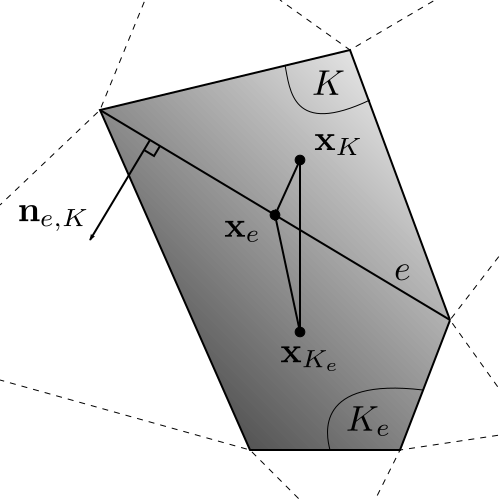
\includegraphics[width=0.25\textwidth]{figs/mesh} \caption{Notations and conventions for mesh discretization and numerical schemes
associated.\label{fig:mesh}}
\end{figure}
\par\end{center}

The SW equations are written in their conservative form as follows:

\begin{equation}
\begin{array}{c}
\text{\ensuremath{\partial}}_{t}\mathbf{U}+\text{\ensuremath{\partial}}_{x}\mathbf{F}(\mathbf{U})+\text{\ensuremath{\partial}}_{y}\mathbf{G}(\mathbf{U})\:=\:\mathbf{S}_{g}(\mathbf{U})+\mathbf{S}_{f}(\mathbf{U})\\
\\
\begin{array}{c}
\mathbf{U}=\begin{bmatrix}h\\
hu\\
hv
\end{bmatrix}\:,\:\mathbf{F}(\mathbf{U})=\begin{bmatrix}hu\\
hu^{2}+{\displaystyle g\frac{h^{2}}{2}}\\
huv
\end{bmatrix}\:,\:\mathbf{G}(\mathbf{U})=\begin{bmatrix}hv\\
huv\\
hv^{2}+{\displaystyle g\frac{h^{2}}{2}}
\end{bmatrix}\:,\\
\\
\mathbf{S}_{g}(z_{b};\mathbf{U})=-g\begin{bmatrix}0\\
h\mathbf{\nabla}z_{b}
\end{bmatrix}\:,\:\mathbf{S}_{f}(\mathbf{U})=-gn^{2}\begin{bmatrix}0\\
{\displaystyle \frac{\left\Vert \mathbf{u}\right\Vert }{h^{1/3}}}\mathbf{u}
\end{bmatrix}
\end{array}
\end{array}\label{eq:sw_cons}
\end{equation}

The term $\mathbf{S}_{g}(z_{b};\mathbf{U})$, resp. $\,\mathbf{S}_{f}(\mathbf{U})$,
denotes the gravitational term, resp. the friction term. 

The expression of $\mathbf{S}_{f}(\mathbf{U})$ above derives from
the Manning-Strickler law, with $n$ the Manning coefficient (friction
coefficient). $n^{2}=K_{S}^{-1}$, $K_{S}$ the Strickler coefficient.
\\

We consider the piecewise constant approximation over mesh cells:

\begin{equation}
\mathbf{U}_{K}={\displaystyle \frac{1}{m_{K}}}\int_{K}\mathbf{U}dK
\end{equation}


\subsection{Schemes for the conservative fluxes }

\subsubsection{Basic principles}

A each time step, the basic principle consists to solve first the
hyperbolic system (\ref{eq:sw_cons}) \emph{without} the source term
$\mathbf{S}_{f}$, next to solve the dynamics system with this source
term $\mathbf{S}_{f}$ only (i.e. $\partial_{t}\boldsymbol{\mathbf{U}}=\mathbf{S}_{f}\left(\mathbf{U}\right)$
). \\

We consider a non unform time grid: $t^{n+1}=t^{n}+\Delta t^{n}$.
We denote by $\mathbf{U}_{K}^{n}$ (resp. by $\mathbf{U}_{K}^{n+1}$)
the piecewise constant approximation of $\mathbf{U}$ at time $t^{n}$
(resp. $t^{n+1}$). Recall that: $\mathbf{U}=\left(h,\boldsymbol{q}\right)=\left(h,h\boldsymbol{u}\right)=(h,q_{x},q_{y})$. 

Let us consider here the hyperbolic system (\ref{eq:sw_cons}) \emph{without}
the source terms $\mathbf{S}_{g}(z_{b};\mathbf{U})$ and $\mathbf{S}_{f}$:
\begin{equation}
\text{\ensuremath{\partial}}_{t}\mathbf{U}+\text{\ensuremath{\partial}}_{x}\mathbf{F}(\mathbf{U})+\text{\ensuremath{\partial}}_{y}\mathbf{G}(\mathbf{U})\:=0
\end{equation}

The current cell (``left cell'') is denoted by $K$. The ``right
cell'' is denoted by $K_{e}$. 

By integrating over $K$, and by applying the Godunov method \cite{Godunov1959},
the semi-discrete scheme for the homogeneous system reads:

\begin{equation}
\mathbf{U}_{K}^{n+1}=\mathbf{U}_{K}^{n}-{\displaystyle \frac{\Delta t^{n}}{m_{K}}\sum_{e\in\partial K}m_{e}}\mathbf{F}_{e}\left(\mathbf{U}_{K}^{n},\mathbf{U}_{K_{e}}^{n},\mathbf{n}_{K}\right)\label{eq:semi-discrete}
\end{equation}

The rotational invariance property of the SW equations (\ref{eq:sw_cons})
allows to reduce this sum of 2D problem to a sum of 1D local Riemann
problems such that: $\mathbf{F}_{e}\left(\mathbf{U}_{K}^{n},\mathbf{U}_{K_{e}}^{n},\mathbf{n}_{K}\right)=\mathbf{R}_{K}^{-1}\hat{\mathbf{F}_{e}}\left(\mathbf{\hat{U}}_{K}^{n},\mathbf{\hat{U}}_{K_{e}}^{n}\right)$
with $\mathbf{\hat{U}}_{K}^{n}=\mathbf{R}_{K}\mathbf{U}_{K}^{n}$
where $\mathbf{R}_{K}$ is the rotation matrix, see e.g. \cite{Toro2001}.
\\

Note that for a computational efficiency in the code, given an edge
$e$, the fluxes are computed in both ways: from left to right and
from right to left. 

\subsubsection{First order scheme}

The HLLC approximate Riemann solver is used. We have, see e.g. \cite{Toro2001}
and references therein: 

\begin{equation}
\left\{ \begin{array}{c}
\begin{array}{c}
\left[\mathbf{\hat{F}}_{e}^{HLLC}\right]_{1,2}={\displaystyle \frac{s_{K_{e}}\left[\mathbf{F}(\hat{\mathbf{U}}_{K})\right]_{1,2}-s_{K}\left[\mathbf{F}(\hat{\mathbf{U}}_{K_{e}})\right]_{1,2}+s_{K}s_{K_{e}}(\left[\hat{\mathbf{U}}_{K_{e}}\right]_{1,2}-\left[\hat{\mathbf{U}}_{K}\right]_{1,2})}{s_{K_{e}}-s_{K}}}\end{array}\\
\left[\mathbf{\hat{F}}_{e}^{HLLC}\right]_{3}=\left[\mathbf{\hat{F}}_{e}^{HLLC}\right]_{1}\hat{v}*\quad\text{with}\quad\hat{v}*=\left\{ \begin{array}{c}
\hat{v}_{K}\quad\text{if}\quad s^{*}\geq0\\
\hat{v}_{K_{e}}\quad\text{if}\quad s^{*}<0
\end{array}\right.
\end{array}\right.\label{eq:hllc}
\end{equation}

The wave speed expression are those proposed in \cite{Vila1986}:
\begin{equation}
\begin{array}{c}
s_{K}=\min\left(0,\hat{u}_{K}-\sqrt{gh_{K}},\hat{u}_{K_{e}}-2\sqrt{gh_{K_{e}}}+\sqrt{gh_{K}}\right)\\
s_{K_{e}}=\max\left(0,\hat{u}_{K_{e}}+\sqrt{gh_{K_{e}}},\hat{u}_{K}+2\sqrt{gh_{K}}-\sqrt{gh_{K_{e}}}\right)
\end{array}\label{eq:hll_waves}
\end{equation}

It has been demonstrated in in \cite{Vila1986} that this insures
$L^{\infty}$ stability, positivity and consistency with entropy condition
under a CFL condition. 

For the intermediate wave speed estimate, following \cite{Toro2001}
we set:

\begin{equation}
s^{*}={\displaystyle \frac{s_{K}h_{K_{e}}\hat{u}_{K_{e}}-s_{K_{e}}h_{K}\hat{u}_{K}-s_{K}s_{K_{e}}(h_{K_{e}}-h_{K})}{h_{K_{e}}(\hat{u}_{K_{e}}-s_{K_{e}})-h_{K}(\hat{u}_{K}-s_{K})}}\label{eq:c_wave}
\end{equation}

The CFL-like condition for the time step $\Delta t^{n}$ is, see e.g.
\cite{Vila2003}:

\begin{equation}
\Delta t^{n}=c\;\min_{K\in\Omega}{\displaystyle \left(\frac{2\;m_{K}}{m_{\partial K}\left(\left\Vert \mathbf{u}_{K}^{n}\right\Vert +\sqrt{gh_{K}^{n}}\right)}\right)}\label{eq:time-step}
\end{equation}

with the constant $c\in\left[0.5,0.8\right]$ in practice. \\

Note that it is usual to introduce a small cut-off water depth $h_{\epsilon}$,
if the velocity components vanishes in order to stabilize the numerical
model or if round-off error generates a negative water depth. With
the complete numerical scheme which is here developed, this cut-off
can be set to a machine epsilon only.

The expressions above are next to be completed by the treatment of
the source term $S_{f}$. 

\subsubsection*{Well-balanced schemes with wet/dry front treatment}

The numerical scheme must preserve the fluid at rest property, that
is the gradient of bathymetry $\nabla z_{b}$ must not provide $\mathbf{u}^{n+1}\ne0$
if $\mathbf{u}^{n}=0$. In the presence of topography gradients (in
particular those perpendicular to the streamlines) the basic topography
gradient $\nabla z_{b}$ discretization in the gravity source term
$\mathbf{S}_{g}\mathbf{\left(U\right)}$ generates spurious velocities.
There is no discrete balance between the hydrostatic pressure and
the gravity source term anymore: ${\displaystyle \nabla\left(gh^{^{2}}/2\right)\neq-gh\nabla z_{b}}$. 

The technique which is employed here is those presented in \cite{Audusse2004,Audusse2005}.
It is based on the following change of variable. 

From now, at left and right sides of edge $e$, the considered water
depth values $h_{\sqcap}^{*}$ are those defined from the ``reconstructed''
topography $z_{e}$ as:

\begin{equation}
\begin{array}{c}
h_{\square}^{*}=\max\left(0,h_{\square}+z_{\square}-z_{e}\right)\\
\text{with}\quad\left\{ \begin{array}{c}
z_{\square}=\eta_{\square}-h_{\square}\\
z_{e}=\max\left(z_{K},z_{K_{e}}\right)
\end{array}\right.
\end{array}\label{eq:hydrostatic_h}
\end{equation}

See Fig. \ref{fig:typical-wb-wet/dry}. 

The conservative variable vector $\mathbf{U}_{e,K}^{n}$ in the semi-discrete
scheme (\ref{eq:semi-discrete-muscl}) is now considered with the
new variable:

\begin{equation}
\mathbf{U}_{\square}^{*}=\begin{bmatrix}h_{\square}^{*}\\
h_{\square}^{*}\mathbf{u}
\end{bmatrix}\label{eq:hydrostatic_h_2-U}
\end{equation}

Note that this new variable $h_{e,K}^{*}$ depends on the bathymetry
values $z_{e,K}$ and $z_{e}$.

The resulting scheme reads: 

\noindent\fbox{\begin{minipage}[t]{1\columnwidth - 2\fboxsep - 2\fboxrule}%
\begin{equation}
\begin{array}{c}
\mathbf{U}_{K}^{n+1}=\mathbf{U}_{K}^{n}-{\displaystyle \frac{\Delta t^{n}}{m_{K}}\sum_{e\in\partial K}m_{e}}\left(\mathbf{F}_{e}(\mathbf{U}_{K}^{*n},\mathbf{U}_{K_{e}}^{*n},\mathbf{n}_{K})+\left.\mathbf{S}_{p}\left(\mathbf{U}_{K}^{n},\mathbf{U}_{K}^{*n};z_{K},z_{K_{e}},\mathbf{n}_{K}\right)\right)\right.\end{array}\label{eq:semi-discrete-wb-order1}
\end{equation}
%
\end{minipage}}

with

\begin{equation}
\begin{array}{c}
\mathbf{S}_{p}\left(\mathbf{U}_{K}^{n},\mathbf{U}_{K}^{*n};z_{K},z_{K_{e}},\mathbf{n}_{K}\right)=\begin{bmatrix}0\\
{\displaystyle \frac{g}{2}}\left(\left(h_{K}^{n}\right)^{2}-\left(h_{K}^{n*}\right)^{2}\right)\mathbf{n}_{K}
\end{bmatrix}\end{array}
\end{equation}

\\

This provides a well-balanced (first order) scheme. 
\begin{center}
\begin{figure}[!tbh]
\centering{}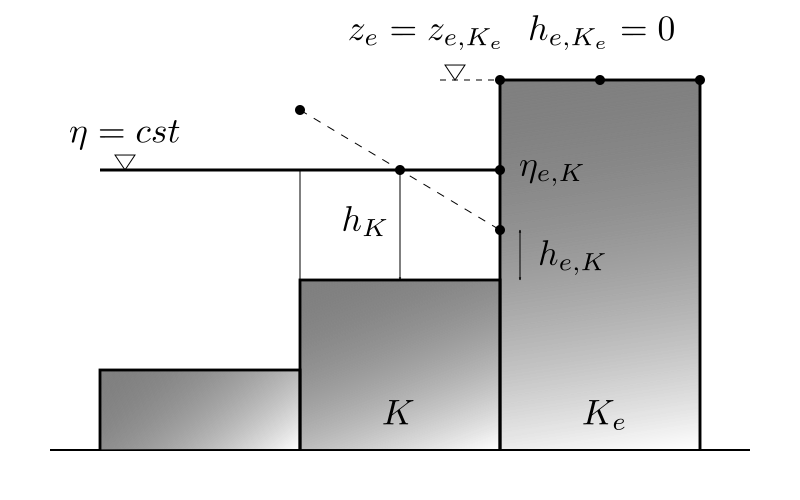
\includegraphics[width=0.4\textwidth]{figs/wb-wet-dry}
\caption{Typical situation of desired well-balanced property in presence of
a wet/dry front. The WS elevation is here denoted by $\eta$. \label{fig:typical-wb-wet/dry}}
\end{figure}
\par\end{center}

\subsubsection{Second order MUSCL scheme }

We here develop a second order scheme based on the concepts of reconstruction
and slope limiting initially introduced by Van Leer in the late 70's. 

A monoslope second order Monotonic Upwind Scheme for Conservation
Laws (MUSCL) scheme is adopted, see e.g. \cite{Chevrier1993,Buffard2010}.
This consists to ``reconstruct'' \emph{locally linear fields by
calculating a vectorial slope $\left[\mathbf{\nabla}\mathbf{U}_{K}^{n}\right]_{i}$
in each cell $K$, for each variable $i$. }

The two ``reconstructed'' conservative variables vectors $\mathbf{U}_{\nabla,K}^{n}$
and $\mathbf{U}_{\nabla,K_{e}}^{n}$ at each side of edge $e$ read
as:

\noindent\fbox{\begin{minipage}[t]{1\columnwidth - 2\fboxsep - 2\fboxrule}%
\begin{equation}
\begin{array}{c}
\mathbf{U}_{\nabla,\square}^{n}=\mathbf{U}_{\square}^{n}+\mathbf{\nabla}\mathbf{U}_{\square}^{n}.\overrightarrow{\mathbf{\mathbf{x}_{\square}\mathbf{x}_{e}}}\end{array}\label{eq:muscl_recons_vector}
\end{equation}
%
\end{minipage}}

with $\square=K$ (``left cell'') or $K_{e}$ (``right cell'').
For $\square=K$, this reads:

\begin{equation}
\begin{array}{c}
\begin{bmatrix}h_{\nabla,K}^{n}\\
h_{\nabla,K}^{n}\mathbf{u}_{\nabla,K}
\end{bmatrix}=\begin{bmatrix}h_{K}^{n}\\
h_{K}^{n}\mathbf{u}_{K}
\end{bmatrix}+\begin{bmatrix}\nabla h_{K}^{n}\\
\nabla(h_{K}^{n}\mathbf{u}_{K})
\end{bmatrix}.\overrightarrow{\mathbf{\mathbf{x}_{\square}\mathbf{x}_{e}}}\end{array}
\end{equation}

These two expressions replace $\mathbf{U}_{K}^{n}$ and $\mathbf{U}_{K_{e}}^{n}$
in the original first order semi-discrete scheme (\ref{eq:semi-discrete})
to evaluate the numerical flux $\mathbf{F}_{e}$. 

From these enriched linear conservative variable, the uncomplete basic
FV scheme reads strictly the same:

\begin{equation}
\mathbf{U}_{K}^{n+1}=\mathbf{U}_{K}^{n}-{\displaystyle \frac{\Delta t^{n}}{m_{K}}\sum_{e\in\partial K}m_{e}}\mathbf{F}_{e}\left(\mathbf{U}_{\nabla,K}^{n},\mathbf{U}_{\nabla,K_{e}}^{n},\mathbf{n}_{K}\right)\label{eq:semi-discrete-muscl}
\end{equation}


\paragraph{Computation of the vectorial slopes}

With a such linear reconstruction, one can expect a scheme with a
second-order accuracy in space (for regular solutions only). To this
end, a least square method is employed to compute the vectorial slopes
for each \emph{primitive} variable denoted by $\mathbf{W}$ . 

\begin{equation}
\mathbf{W}=\left[h,u,v\right]^{T}
\end{equation}

Let us defined the sum of squares for each $i$, $i=1,\dots,3$:

\begin{equation}
\begin{array}{c}
E_{i}\left(\left[\widetilde{\mathbf{\nabla}\mathbf{W}_{K}^{n}}\right]_{i}\right)={\displaystyle \sum_{e\in\partial K}\left(\left[\mathbf{W}_{K_{e}}^{n}\right]_{i}-\left(\left[\mathbf{W}_{K}^{n}\right]_{i}+\left[\mathbf{\nabla}\mathbf{W}_{K}^{n}\right]_{i}.\overrightarrow{\mathbf{x}_{K}\mathbf{x}_{K_{e}}}\right)\right)^{2}}\end{array}\label{eq:ls_muscl}
\end{equation}

Each term $E_{i}\left(\left[\widetilde{\mathbf{\nabla}\mathbf{W}_{K}^{n}}\right]_{i}\right)$
is minimized (as the solution of simple $2\times2$ linear systems).
\\

This method represents a good alternative among others to find the
hyperplane \cite{Chevrier1993,Haider2009} because of its accuracy
and robustness independently to the number of neighbours. This is
an important property as it will be shown later with the present wet/dry
front treatment.

\paragraph{Limitation of the vectorial slopes}

In order to prevent large numerical instabilities, the computed vectorial
slopes above need to be limited.

\textbf{Maximum Principle (MP) limiter}

A first method consists to apply the Maximum Principle (MP) to the
two edge (unlimited) reconstructed primitive variables calculated
from (\ref{eq:muscl_recons_vector}) and (\ref{eq:ls_muscl}). 

Then the limited reconstructed variables $\mathbf{W}_{\nabla,K}^{n}$
and $\mathbf{W}_{\nabla,K_{e}}^{n}$ are defined as:

\begin{equation}
\min\left(\mathbf{W}_{K}^{n},\mathbf{W}_{K_{e}}^{n}\right)\leq\mathbf{W}_{\nabla,K}^{n}\mbox{ and }\mathbf{W}_{\nabla,K_{e}}^{n}\leq\max\left(\mathbf{W}_{K}^{n},\mathbf{W}_{K_{e}}^{n}\right)
\end{equation}

This is the so-called the MP limiter.

In practice, this method generates moderate oscillations at solution
singularities, whereas diffusion is minimized comparatively to other
classic limiters like Minmod or Van Albada, see also e.g. \cite{Audusse2005,Nikolos2009,Delis2011,Delis2013}.
\\

It is worth to point out that generation of new extremas in presence
of\textit{\emph{ wet/dry fronts}} can break the mass conservation,
and in this case\emph{ the scheme is no longer positive.}


\subsubsection*{Well-balanced schemes with wet/dry front treatment}

Following \cite{Audusse2004,Audusse2005}, this issue is solved by
evaluating the vectorial slope for the water surface elevation $H$
rather than for the water height $h$. A new vectorial slope for the
variable $\eta=h+z$ is first calculated in addition to the primitive
variables ones. 

As previously, the so-called hydrostatic reconstructed water depth
$h_{e,K}^{*}$ is defined from the reconstructed topography $z_{e}$
at edge $e$ as:

\begin{equation}
\begin{array}{c}
h_{\nabla,\square}^{*}=\max\left(0,h_{\nabla,\square}+z_{\square}-z_{e}\right)\\
\text{with}\quad\left\{ \begin{array}{c}
z_{\square}=\eta_{\square}-h_{\nabla,\square}\\
z_{e}=\max\left(z_{K},z_{K_{e}}\right)
\end{array}\right.
\end{array}\label{eq:hydrostatic_h_nabla}
\end{equation}

with $\square=K$ (``left cell'') or $K_{e}$ (``right cell'').
See Fig. \ref{fig:typical-wb-wet/dry}. 

The conservative variable vector $\mathbf{U}_{K}^{n}$ in the semi-discrete
scheme (\ref{eq:semi-discrete-muscl}) is now considered with the
new variable:

\begin{equation}
\mathbf{U}_{\nabla,\square}^{*}=\begin{bmatrix}h_{\nabla,\square}^{*}\\
(h^{*}\mathbf{u})_{\nabla,\square}
\end{bmatrix}
\end{equation}

Let us write the \emph{second order scheme in space only} while considering
the basic explicit Euler time scheme for sake of clarity. This reads:

\noindent\fbox{\begin{minipage}[t]{1\columnwidth - 2\fboxsep - 2\fboxrule}%
\begin{equation}
\mathbf{U}_{K}^{n+1}=\mathbf{U}_{K}^{n}-{\displaystyle \frac{\Delta t^{n}}{m_{K}}\sum_{e\in\partial K}m_{e}}\mathbf{L}_{e}\left(\mathbf{U}_{K}^{n},\mathbf{U}_{\nabla,K}^{n},\mathbf{U}_{\nabla,K}^{*n};\mathbf{U}_{\nabla,K_{e}}^{*n};z_{K},z_{K_{e}},\mathbf{n}_{K}\right)\label{eq:semi-discrete-wb-order2}
\end{equation}
\\
\begin{equation}
\mathbf{L}_{e}\equiv\mathbf{L}_{e}\left(\mathbf{U}_{K}^{n},\mathbf{U}_{\nabla,K}^{n},\mathbf{U}_{\nabla,K}^{*n};\mathbf{U}_{\nabla,K_{e}}^{*n};z_{K},z_{K_{e}},\mathbf{n}_{K}\right)=\mathbf{F}_{e}\left(\mathbf{U}_{\nabla,K}^{*n};\mathbf{U}_{\nabla,K_{e}}^{*n};\mathbf{n}_{K}\right)+\mathbf{S}_{p}\left(\mathbf{U}_{\nabla,K}^{n},\mathbf{U}_{\nabla,K}^{*n};z_{K},z_{K_{e}},\mathbf{n}_{K}\right)+\mathbf{S}_{g}\left(\mathbf{U}_{K}^{n},\mathbf{U}_{\nabla,K}^{n},z_{K},\mathbf{n}_{K}\right)\label{def:Le}
\end{equation}

with

\begin{equation}
\begin{array}{c}
\mathbf{S}_{p}\left(\mathbf{U}_{\nabla,K}^{n},\mathbf{U}_{\nabla,K}^{*n};z_{K},z_{K_{e}},\mathbf{n}_{K}\right)=\begin{bmatrix}0\\
{\displaystyle \frac{g}{2}}\left(\left(h_{\nabla,K}^{n}\right)^{2}-\left(h_{K}^{n*}\right)^{2}\right)\mathbf{n}_{K}
\end{bmatrix}\end{array}
\end{equation}

and the gravitational uncentered corrective term: 

\textbf{
\begin{equation}
\begin{array}{c}
\mathbf{S}_{g}\left(\mathbf{U}_{K}^{n},\mathbf{U}_{\nabla,K}^{n};z_{K},\mathbf{n}_{K}\right)=\begin{bmatrix}0\\
{\displaystyle \frac{g}{2}}\left(h_{\nabla,K}^{n}+h_{K}^{n}\right)\left(z_{\nabla,K}-z_{K}\right)\mathbf{n}_{K}
\end{bmatrix}\end{array}
\end{equation}
}

\textbf{}%
\end{minipage}}

However, numerical experiments show that this scheme is not stable
at wet/dry fronts perpendicular to the flow streamlines.

\subsubsection*{}

\subsection{Splitting and friction source term}

The friction source term is taken into account in the complete SW
system by deriving a splitting method. This may be viewed as prediction-correction
time scheme too. We refer to \cite{Toro2001} Chapter 12. \\

\emph{We denote here by $\bar{\mathbf{U}}_{K}^{n+1}$ the FV solution
at time $t^{n+1}$ of the (well-balanced) scheme, either first or
second order, of the SW system with the gravitational term $\mathbf{S}_{g}$
but without the friction term $\mathbf{S}_{f}$. }\\
\\
The notation $\bar{}$ should not be mixed up with depth-averaging...

Recall that we denote: $\mathbf{U}=\left(h,h\boldsymbol{u}\right)^{T}$. 

\subsubsection*{Prediction- correction scheme / splitting scheme }

At each time step, from $n$ to $n+1$, 
\begin{itemize}
\item \textbf{Step 1: }computation of $\bar{\mathbf{U}}^{n+1}$, solution
of the conservative SW system, i.e. the SW system \emph{without $S_{f}$},
i.e. the FV solution of the following system: 
\begin{equation}
\partial_{t}\boldsymbol{U}+\partial_{x}\boldsymbol{F}\left(\boldsymbol{U}\right)+\partial_{y}\boldsymbol{G}\left(\boldsymbol{U}\right)=\mathbf{S}_{g}\left(\boldsymbol{U}\right)\label{eq:substep_SWE_with_grav_term}
\end{equation}
\end{itemize}
Recall that the discrete form of Eq. \ref{eq:substep_SWE_with_grav_term}
reads: for all $K$,

\noindent\fbox{\begin{minipage}[t]{1\columnwidth - 2\fboxsep - 2\fboxrule}%
First order case:

\begin{align}
\mathbf{\bar{U}}_{K}^{n+1} & =\mathbf{U}_{K}^{n}-\Delta t^{n}\left[{\displaystyle \frac{1}{m_{K}}\sum_{e\in\partial K}m_{e}}\left(\mathbf{F}_{e}(\mathbf{U}_{K}^{*n},\mathbf{U}_{K_{e}}^{*n},\mathbf{n}_{K})+\left.\mathbf{S}_{p}\left(\mathbf{U}_{K}^{n},\mathbf{U}_{K}^{*n};z_{K},z_{K_{e}},\mathbf{n}_{K}\right)\right)\right.\right]\label{eq:semi-implicit-friction-1}
\end{align}
%
\end{minipage}}

\noindent\fbox{\begin{minipage}[t]{1\columnwidth - 2\fboxsep - 2\fboxrule}%
Second order case:

\begin{align}
\mathbf{\bar{U}}_{K}^{n+1} & =\mathbf{U}_{K}^{n}-\Delta t^{n}\left[{\displaystyle \frac{1}{m_{K}}\sum_{e\in\partial K}m_{e}}\left(\mathbf{F}_{e}\left(\mathbf{U}_{\nabla,K}^{*n};\mathbf{U}_{\nabla,K_{e}}^{*n};\mathbf{n}_{K}\right)+\mathbf{S}_{p}\left(\mathbf{U}_{\nabla,K}^{n},\mathbf{U}_{\nabla,K}^{*n};z_{K},z_{K_{e}},\mathbf{n}_{K}\right)+\mathbf{S}_{g}\left(\mathbf{U}_{K}^{n},\mathbf{U}_{\nabla,K}^{n},z_{K},\mathbf{n}_{K}\right)\right)\right]\label{eq:semi-implicit-friction}
\end{align}
%
\end{minipage}}
\begin{itemize}
\item \textbf{Step 2: }given the ''predicted value'' $\bar{\mathbf{U}}^{n+1}$,
compute $\mathbf{U}^{n+1}$ solution of:
\begin{equation}
\partial_{t}\boldsymbol{\mathbf{U}}=\mathbf{S}_{f}\left(\mathbf{U}\right)\label{eq:substep_friction_term}
\end{equation}
\end{itemize}
\textbf{Expression of $\mathbf{U^{n+1}}$ in the first order case}

General schemes (explicit, implicit or semi-implicit ones) including
the friction source term $\mathbf{S}_{f}$ in the discretization of
the model (Eq. \ref{eq:sw_cons}) can be written as: for all $K$,

\begin{align}
\mathbf{U}_{K}^{n+1} & =\mathbf{\bar{U}}_{K}^{n+1}+\Delta_{t}^{n}\mathbf{S}_{f}\left(\mathbf{\bar{U}}_{K}^{n+1},\mathbf{\bar{U}}_{K_{e}}^{n+1}\right)\label{eq:semi-implicit-friction-1-1}
\end{align}

Note that this splitting scheme is consistent at first order in $\Delta t$
with the complete SWE. Splitting scheme second order in time is possible;
it is not detailed later. 

In the case of the Manning-Strickler law, the friction term reads:
$\mathbf{S}_{f}=-gn^{2}\left[\begin{array}{c}
0\\
\frac{\left|\bar{\boldsymbol{u}}\right|}{h^{\frac{1}{3}}}\boldsymbol{\bar{u}}
\end{array}\right]$. 

Therefore the equation to be solved (Eq. \ref{eq:substep_friction_term})
reads:
\begin{equation}
\partial_{t}\left(\begin{array}{c}
h\\
h\boldsymbol{\bar{u}}
\end{array}\right)=-gn^{2}\left(\begin{array}{c}
0\\
\frac{\left|\bar{\boldsymbol{u}}\right|}{h^{\frac{1}{3}}}\boldsymbol{\bar{u}}
\end{array}\right)\label{eq:7}
\end{equation}

Since the friction source term $\mathbf{S}_{f}$ is zero in the mass
conservation equation, we remark that $h^{n+1}=\bar{h}^{n+1}$.

As a consequence, we consider the non-zero momentum component only:
\begin{equation}
\partial_{t}\left(h\boldsymbol{\bar{u}}\right)=-gn^{2}\frac{\left|\bar{\boldsymbol{u}}\right|}{h^{\frac{1}{3}}}\boldsymbol{\bar{u}}\label{eq:8}
\end{equation}

Let us consider \emph{the implicit scheme} (implicit in $u$ and $h$):
\begin{equation}
\frac{h^{n+1}\boldsymbol{u}^{n+1}-h^{n+1}\bar{\boldsymbol{u}}^{n+1}}{\Delta t^{n}}=-gn^{2}\frac{\left|\boldsymbol{u}^{n+1}\right|\boldsymbol{u}^{n+1}}{\left(h^{n+1}\right)^{\frac{1}{3}}}
\end{equation}

This implies that:

\begin{equation}
\left|\boldsymbol{u}^{n+1}\right|\boldsymbol{u}^{n+1}+\frac{\left(h^{n+1}\right)^{\frac{4}{3}}}{\Delta t^{n}gn^{2}}\left(\boldsymbol{u}^{n+1}-\bar{\boldsymbol{u}}^{n+1}\right)=0
\end{equation}

Let us set $c=\frac{\left(h^{n+1}\right)^{\frac{4}{3}}}{\Delta t^{n}gn^{2}}$.
$c\geq0$.

Note that $\left|\boldsymbol{u}^{n+1}\right|\boldsymbol{u}^{n+1}+c\boldsymbol{u}^{n+1}=c\bar{\boldsymbol{u}}^{n+1}$.
Therefore for non vanishing velocities, it exists $\alpha\in\left]0,1\right]$
such that: $\boldsymbol{u}^{n+1}=\alpha\bar{\boldsymbol{u}}^{n+1}$. 

Adopting these notations, we obtain: $\left|\bar{\boldsymbol{u}}^{n+1}\right|\bar{\boldsymbol{u}}^{n+1}\alpha^{2}+c\bar{\boldsymbol{u}}^{n+1}\alpha-c\bar{\boldsymbol{u}}^{n+1}=0$.
This simplifies to:
\begin{equation}
\left|\bar{\boldsymbol{u}}^{n+1}\right|\alpha^{2}+c\thinspace\alpha-c=0
\end{equation}

Since $\alpha\geq0$, the root of this quadratic equation reads:

\begin{equation}
\alpha=\frac{-c+\sqrt{c^{2}+4c\left|\bar{\boldsymbol{u}}^{n+1}\right|}}{2\left|\bar{\boldsymbol{u}}^{n+1}\right|}\label{eq:alpha}
\end{equation}

Let us define the function $\varepsilon=\frac{1}{c}\left|\bar{\mathbf{u}}^{n+1}\right|=\Delta t^{n}gn^{2}\frac{\left|\bar{\mathbf{u}}^{n+1}\right|}{\left(h^{n+1}\right)^{4/3}}$.

Observe that $\varepsilon=O\left(\Delta t^{n}\right)$, also $\varepsilon=O\left(\frac{\left|\bar{\mathbf{u}}^{n+1}\right|}{\left(h^{n+1}\right)^{4/3}}\right)$.

By adopting this notation, the expression (\ref{eq:alpha}) of $\alpha$
reads: $\alpha=\frac{\sqrt{1+4\epsilon}-1}{2\epsilon}$. 

After some rearrangements, we obtain:

\begin{align}
\alpha & =\frac{2}{1+\sqrt{1+4\varepsilon}}\label{eq:alpha_epsilon}
\end{align}
At 1st order in $\epsilon$, we get: $\alpha\sim\left({\displaystyle \frac{1}{1+\epsilon/4}}\right)\sim1-\epsilon/4$.

Finally, we obtain:

\begin{equation}
\boldsymbol{u}^{n+1}=\left({\displaystyle \frac{2\left(h^{n+1}\right)^{2/3}}{\left(h^{n+1}\right)^{2/3}+\sqrt{\left(h^{n+1}\right)^{\frac{4}{3}}+4\Delta t^{n}gn^{2}\left|\bar{\mathbf{u}}^{n+1}\right|}}}\right)\bar{\boldsymbol{u}}^{n+1}\label{eq:u_n+1_final}
\end{equation}

The final expression of the first order scheme is:

\noindent\fbox{\begin{minipage}[t]{1\columnwidth - 2\fboxsep - 2\fboxrule}%
\begin{equation}
\mathbf{U}_{K}^{n+1}=\left(\begin{array}{c}
h^{n+1}\\
h^{n+1}\boldsymbol{u}^{n+1}
\end{array}\right)=\begin{bmatrix}\begin{array}{c}
\bar{h}^{n+1}\\
h^{n+1}\bar{\mathbf{u}}^{n+1}\left({\displaystyle \frac{2\left(\bar{h}^{n+1}\right)^{2/3}}{\left(\bar{h}^{n+1}\right)^{2/3}+\sqrt{\left(\bar{h}^{n+1}\right)^{\frac{4}{3}}+4\Delta t^{n}gn^{2}\left|\bar{\mathbf{u}}^{n+1}\right|}}}\right)
\end{array}\end{bmatrix}\label{eq:Un+1}
\end{equation}
%
\end{minipage}}

With $\left|\bar{\mathbf{u}}^{n+1}\right|$ the solution of Eq. \ref{eq:semi-implicit-friction-1}
. 

This is the first order scheme implemented into the code.

Note that the friction coefficient $n$ may depend on the depth $h$
like e.g. $n\equiv n(\alpha,\beta;h)=\alpha h^{\beta}$.

\subsubsection*{Expression of $\mathbf{U^{n+1}}$ in the second order case }

In order to obtain a globally second order scheme, a higher-order
time stepping scheme is needed. 

A first possibility would be to replace the explicit splitted step
for $\mathbf{S}_{f}$ in the classical second order SSP-RK2 method,
see e.g. \cite{Gottlieb2001}.

This time splitting strategy is stable and preserves positivity, however
it is first order only !...\\

In order to derive an \emph{actual second order scheme} with an full
implicit discretization of the source term, Pareschi and Russo in
\cite{Pareschi2005} derive an IMplicit-EXplicit (IMEX) Runge-Kutta
method for hyperbolic conservation laws with stiff relaxation terms. 

Here we consider the scheme named IMEX-SSP(3,2,2). This provides the
following scheme:

\noindent\fbox{\begin{minipage}[t]{1\columnwidth - 2\fboxsep - 2\fboxrule}%
\begin{equation}
\begin{array}{lcll}
\mathbf{U}_{K}^{(1)} & = & \mathbf{U}_{K}^{n} & +{\displaystyle \frac{\Delta t^{n}}{2}}\mathbf{S}_{f}(\mathbf{U}_{K}^{(1)},\mathbf{U}_{K}^{n})\\
\mathbf{U}_{K}^{(2)} & = & 2\mathbf{U}_{K}^{n}-\mathbf{U}_{K}^{(1)} & +{\displaystyle \frac{\Delta t^{n}}{2}}\mathbf{S}_{f}(\mathbf{U}_{K}^{(2)},\mathbf{U}_{K}^{n})\\
\mathbf{U}_{K}^{(3)} & = & \mathbf{U}_{K}^{n} & +\Delta t^{n}\mathbf{L}_{e}(\mathbf{U}_{K}^{(2)})\\
\mathbf{U}_{K}^{(4)} & = & \mathbf{U}_{K}^{(1)}+\mathbf{U}_{K}^{(2)}+\mathbf{U}_{K}^{(3)}-2\mathbf{U}_{K}^{n} & +{\displaystyle \frac{\Delta t^{n}}{2}}\mathbf{S}_{f}(\mathbf{U}_{K}^{(4)},\mathbf{U}_{K}^{n})\\
\mathbf{U}_{K}^{(5)} & = & \mathbf{U}_{K}^{n} & +\Delta t^{n}\mathbf{L}_{e}(\mathbf{U}_{K}^{(4)})\\
\mathbf{U}_{K}^{n+1} & = & {\displaystyle \frac{1}{2}}\left(\mathbf{U}_{K}^{(5)}-\mathbf{U}_{K}^{(3)}\right)+\mathbf{U}_{K}^{(4)}
\end{array}
\end{equation}
%
\end{minipage}}

with $\mathbf{L}_{e}(\mathbf{U}_{K}^{(l)})\equiv\mathbf{L}_{e}\left(\mathbf{U}_{K}^{(l)},\mathbf{U}_{\nabla,K}^{(l)},\mathbf{U}_{\nabla,K}^{*(l)};\mathbf{U}_{\nabla,K_{e}}^{*(l)};z_{K},z_{K_{e}},\mathbf{n}_{K}\right)$
defined by (\ref{def:Le}). 

The three stages implicit part of this time splitting is a DIRK scheme
\cite{Pareschi2005} respecting A-stability, L-stability. It is stiffly
accurate ($R(\infty)=0$) , see \cite{Hairer2004}. Such stability
properties enable to deal with wet/dry fronts where the friction source
term $\mathbf{S}_{f}$ is extremely stiff. ($\mathbf{S}_{f}$ stiff
because the water depth vanishes). 

Moreover this version of the DIRK scheme has been found important
to treat non trivial boundaries conditions without any special correction.\\
\\
This is the second order scheme implemented into the code.

\subsection{Boundary conditions}

Recall that the current cell is denoted by $K$ (``left cell'').
It is here a in-domain cell. Here $K_{e}$ denotes the ghost cell
(``right cell''). 

The basic idea to impose the boundary conditions is to define ghost
conservative vectors: $\mathbf{U}_{K_{e}}^{G}$ for the first order
scheme and $\mathbf{U}_{\nabla,K_{e}}^{G}$ for the second order for
an edge $e$ at the boundary of $\Omega$.

Note that it is not straightforward to impose a numerical flux value
e.g. $Q_{in}(t)$.\\
 

Let $\mathbf{U}_{K_{e}}^{G}$ be the value of $\mathbf{U}$ in a virtual
(ghost) cell $K_{e}$ adjacent to the boundary $\partial\Omega$.

\paragraph*{Wall B.C. }

The following local Riemann problems are solved: 

\begin{equation}
\left\{ \begin{array}{ccc}
h_{K_{e}}^{G} & = & h_{K}+(z_{K}-z_{K_{e}})\\
\hat{u}_{K_{e}}^{G} & = & -\hat{u_{K}}\\
\hat{v}_{K_{e}}^{G} & = & \hat{v}_{K}
\end{array}\right.\label{eq:bc_wall}
\end{equation}


\paragraph*{Imposed discharge: inflow discharge or rating curve at outflow}

To impose $Q_{\text{in}}$ at $\Gamma_{in}$ or a rating curve $Q_{out}(\eta)$
at $\Gamma_{out}$, whatever the fluid rheology, the following primitive
variables ghost values are set in the local Riemann solver:

\begin{equation}
\left\{ \begin{array}{ccc}
h_{K_{e}}^{G} & = & h_{K}\\
\hat{u}_{K_{e}}^{G} & = & {\displaystyle \frac{Q_{\text{user}}h_{K}^{{\displaystyle \nicefrac{2}{3}}}}{\underset{e\in\Gamma_{\text{in}}}{\sum}h_{e,K}^{{\displaystyle \nicefrac{5}{3}}}m_{e}}}\\
\hat{v}_{K_{e}}^{G} & = & \hat{v}_{K}
\end{array}\right.\label{eq:bc_in}
\end{equation}

$Q_{user}$denotes either a given hydrogram $Q_{in}(t)$ ($m^{3}/s)$,
or a rating curve $Q_{out}(\eta)$. 

The latter may be linearly interpoled function from tabulated values. 

 If the wetted cross-section at the boundary is not rectangular,
the computed discharge value in $K$ is a-priori not equal to the
imposed value $Q_{\text{in}}$ !...

To overcome this issue, a feedback process is applied on the ghost
bathymetry $z_{K_{e}}$ as follows:

\begin{equation}
z_{K_{e}}^{\text{new}}\ =\ z_{K_{e}}^{\text{old}}+cst\left(\mathbf{F}_{e}(\mathbf{U}_{K}^{n},\mathbf{U}_{K_{e}}^{n};\mathbf{n}_{e,K})-q_{K_{e}}^{G}\right)\label{eq:bc_in_correc}
\end{equation}

where: $q_{K_{e}}^{G}=h_{K}u_{K_{e}}^{G}$($m^{2}/s)$ and $cst$
can be changed ($cst=0.1$ by default). 

This process correct the ghost bathymetry $z_{b}^{G}$ \emph{at each
time step} to finally converge to a value implying that the mass flux
$\mathbf{F}_{e}^{h}(\mathbf{U}_{K}^{n},\mathbf{U}_{K_{e}}^{n},\mathbf{n}_{e,K})$
is stricly equal to the imposed lineic discharge $\hat{q}_{K_{e}}^{G}$.

\paragraph*{Depth imposed}

In order to control the depth value at a boundary e.g. at $\Gamma_{out}$,
the following values are considered: 

\begin{equation}
\left\{ \begin{array}{ccc}
h_{K_{e}}^{G} & = & h_{\text{user}}\\
\hat{u}_{K_{e}}^{G} & = & \hat{u}_{K}+2\sqrt{g}\left(\sqrt{h_{user}}-\sqrt{h_{K}}\right)\\
\hat{v}_{K_{e}}^{G} & = & \hat{v}_{K}
\end{array}\right.\label{eq:bc_out}
\end{equation}


\paragraph*{Second-order case}

In the case of the second-order scheme, one has the ``reconstructed''
variable $\mathbf{U}_{\nabla,K_{e}}^{G}$; $\mathbf{U}_{K_{e}}^{G}$
is first used in the least square method (\ref{eq:ls_muscl}) to compute
the vectorial slope in the interior cell $K$. 

The conditions (\ref{eq:bc_wall}), (\ref{eq:bc_in}) and (\ref{eq:bc_out})
are then used a second time replacing $\mathbf{U}_{K}$ by $\mathbf{U}_{\nabla,K}$
to obtain $\mathbf{U}_{\nabla,K_{e}}^{G}$. 

Finally, the hydrostatic reconstructed depth $h_{K_{e}}^{^{*},G}$
and $h_{\nabla,K_{e}}^{^{*},G}$ are calculated in the same way through
equations (\ref{eq:hydrostatic_h}) and (\ref{eq:hydrostatic_h_nabla})
with $z_{\nabla,K_{e}}^{G}=z_{\nabla,K_{e}}$.

\section{Validation}

This section is dedicated to the validation of the numerical schemes
implemented in the \DassFlow{} software presenting several challenging
and relevant test cases in context of hydraulic and environnemental
studies : dam break, channel and run-up problems with dynamic wet/dry
fronts and considering non-linear friction. We will show the formally
global second-order convergence in space and time of our SW numerical
model with the Manning-Strickler friction source term as the robust
treatment of wet/dry fronts.

In order to quantify the numerical errors, we define these relative
error norms,

\begin{equation}
\begin{array}{c}
e_{p}(x)={\displaystyle {\displaystyle \frac{\Vert x^{\text{num}}-x^{\text{exact}}\Vert_{p}}{\Vert x^{\text{exact}}\Vert_{p}}\quad}},\quad e_{p}^{T}(x)={\displaystyle \frac{1}{T}\int_{0}^{T}e_{p}(x)\ dt}\\
\\
\Vert x\Vert_{p}=\left({\displaystyle \sum_{K\in\Omega}m_{K}\left|x_{K}\right|^{p}}\right)^{1/p}
\end{array}
\end{equation}

where $x^{\text{num}}$ is the numerical solution with $n$ cells
of discretization and $x^{\text{exact}}$ is the analytical solution
of the test case or the converge reference solution when the analytical
solution is not known ($x_{i}^{\text{exact}}$ is properly numerically
integrated with desired accuracy in sense of used Finite Volume schemes).

\subsection{Water at rest}

We consider in a box $1000$ meter long a zero bed elevation, ramdomly
perturbated cell by cell with a maximum amplitude of $1\ m$,

\begin{equation}
z_{b}=r\quad\text{with}\quad r\in\left[-1,1\right]
\end{equation}

If the simualtion is initialized with a water elevation of zero, i.e.
$z_{b}+h=0$, the resulting ``lake'' should stay at rest. After
a simulation time of $3600\ s$, the results with different schemes
are showed in the Fig.(\ref{fig:water-at-rest}). The norms of the
final velocities are given in the Tab.\ref{tab:Water-at-rest}.

\begin{center}
\begin{table}[!tbh]
\begin{centering}
\begin{tabular}{>{\centering}p{0.05\textwidth}>{\centering}p{0.1\textwidth}>{\centering}p{0.1\textwidth}>{\centering}p{0.1\textwidth}>{\centering}p{0.1\textwidth}>{\centering}p{0.1\textwidth}>{\centering}p{0.1\textwidth}}
\toprule 
 & 1�order & 1�order / WB-A & 2�order & 2�order / MP limiter / WB-A / CFL 0.5 & 2�order/ MP limiter / WB-A / CFL 0.25 & 2�order/ Barth limiter / WB-A\tabularnewline
\midrule 
$\Vert\mathbf{u}\Vert_{\infty}$ & $2.30$ & $1.04\ 10^{-13}$ & $2.23$ & $1.45\ 10^{-2}$ & $9.66\ 10^{-14}$ & $7.66\ 10^{-14}$\tabularnewline
\midrule 
$\Vert\mathbf{u}\Vert_{1}$ & $1.14$ & $6.92\ 10^{-16}$ & $0.95$ & $1.95\ 10^{-5}$ & $9.40\ 10^{-16}$ & $6.97\ 10^{-16}$\tabularnewline
\bottomrule
\end{tabular}
\par\end{centering}
\caption{Water at rest test case, absolute infinity and $L_{1}$ norms of the
final velocities.\label{tab:Water-at-rest}}
\end{table}
\par\end{center}

\begin{center}
\begin{figure}[!tbh]
\begin{centering}
\includegraphics[width=0.5\textwidth,bb = 0 0 200 100, draft, type=eps]{/home/leo/Desktop/SVN/dassflow-2d/trunk/doc/figs/water_at_rest_first.pdf}\includegraphics[width=0.5\textwidth,bb = 0 0 200 100, draft, type=eps]{/home/leo/Desktop/SVN/dassflow-2d/trunk/doc/figs/water_at_rest_first_b1.pdf}
\par\end{centering}
\centering{}\includegraphics[width=0.5\textwidth,bb = 0 0 200 100, draft, type=eps]{/home/leo/Desktop/SVN/dassflow-2d/trunk/doc/figs/water_at_rest_muscl_b1_cfl_0.5.pdf}\includegraphics[width=0.5\textwidth,bb = 0 0 200 100, draft, type=eps]{/home/leo/Desktop/SVN/dassflow-2d/trunk/doc/figs/water_at_rest_muscl_b1_b.pdf}\caption{Water at rest test case, final water depth and velocities; (up-left)
first order scheme; (up-right) well-balanced first order scheme; (down-left)
well-balanced second order scheme with the MP limiter and a CFL number
of $0.5$; (down-right) well-balanced second order scheme with the
Barth limiter.\label{fig:water-at-rest}}
\end{figure}
\par\end{center}

\subsection{Parabolic bowl with linear friction}

Analytical solutions of the nonlinear SW equations considering a linear
friction and a parabolic bottom topography were derived by Sampson
\cite{Sampson2006}, following the work of Thacker \cite{Thacker1981},
by considering a linear friction in replacement of Coriolis force.
These solutions involve a flat surface oscillating motion with wet/dry
fronts, decaying over time because of friction. It gives a very popular
test for a SW numerical solver \cite{Audusse2005,Liang2009,Song2011,Kesserwani2012,Hou2013}.
The solution is,

\begin{equation}
\begin{array}{ccl}
\eta(x,t) & = & h_{0}+{\displaystyle \frac{a^{^{2}}B^{^{2}}e^{-\tau t}}{8g^{^{2}}h_{0}}\left({\displaystyle -s\tau}\sin2st+\left({\displaystyle \frac{\tau^{2}}{4}-s^{^{2}}}\right)\cos2st\right)}\\
 &  & -{\displaystyle \frac{B^{2}e^{-\tau t}}{4g}-{\displaystyle \frac{e^{-\tau t/2}}{g}}\left(Bs\cos st+{\displaystyle \frac{\tau B}{2}\sin st}\right)x}\\
\\
u(x,t) & = & Be^{-\tau t/2}\sin st
\end{array}
\end{equation}

with $p=\sqrt{{\displaystyle 8gh_{0}}}/a$ and $s={\displaystyle \sqrt{p^{2}-\tau^{2}}/2}$
(and then valid if $p>\tau$). We choose two set of parameters,

\begin{equation}
\text{set 1}\ \ \left\{ \begin{array}{ccc}
h_{0} & = & 10\ m\\
a & = & 3000\ m\\
B & = & 5\ m.s^{-1}\\
\tau & = & 0.001\ s^{-1}
\end{array}\qquad\right.\text{set 2}\ \ \left\{ \begin{array}{ccc}
h_{0} & = & 1\ m\\
a & = & 30\ m\\
B & = & 1\ m.s^{-1}\\
\tau & = & 0.2\ s^{-1}
\end{array}\right.\label{eq:set-bowl}
\end{equation}

The first one corresponding to the classic parameters chosen into
litterature as in \cite{Liang2009,Kesserwani2012}. The Fig.(\ref{fig:bowl_norms})
shows the calculated relative error norms $e_{1}^{T}(h)$ with this
first set of parameters using the MP limiter for the second order
well-balanced scheme. One can observe the correct convergence behavior
of all well-balance schemes and demonstrate that the moving wet-dry
fronts are robustly captured (a cut-off water depth $h_{\epsilon}\in\left[10^{-4},10^{-8}\right]$
have been used for these simulations in order to find a linear convergence
behavior in log-log scale). A rate of convergence of approximatively
1.5 is found for the second-order well-balance scheme with the hybrid
SSP-RK2 time splitting as with the IMEX time splitting (It is found
a relative error norm $e_{1}^{T}(h)\simeq2.10^{-3}$ for $n=100$
which is approximatively the same in \cite{Liang2009}). This loss
of second order accuracy is most probably due to the presence of the
two moving wet/dry fronts introducing singularities in the solution.
But a most interesting observation is that there is no major difference
between the two time splitting strategy despite the fact that the
hybrid RK2 is first order accurate and the IMEX second order accurate,
except maybe for very fine meshes. This demonstrates that the spatial
consistency error is greater than the time one despite the accuracy
slopes difference. If simulations are performed now with the second
set of paramaters (\ref{eq:set-bowl}), then it is obtained a significant
difference between the two time splitting methods Fig.(\ref{fig:bowl_norms}).
After an asymptotic first order behavior for coarse meshes, the hybrid
RK2 time splitting gives a rate of convergence of 1 and the IMEX time
splitting maintains the same 1.5 rate of convergence obtained with
the first classic set of parameters (\ref{eq:set-bowl}).

\begin{center}
\begin{figure}[tbh]
\centering{}\includegraphics[width=0.5\textwidth,bb = 0 0 200 100, draft, type=eps]{/home/leo/Desktop/SVN/dassflow-2d/trunk/doc/figs/thacker_conv.pdf}\includegraphics[width=0.5\textwidth,bb = 0 0 200 100, draft, type=eps]{/home/leo/Desktop/SVN/dassflow-2d/trunk/doc/figs/thacker_conv_splitting_error.pdf}\caption{(left) Rate of convergence for the norm $e_{1}^{T}(h)$ with set 1
of physical parameters, $n$ is the cells number (right) Same with
set 2.\label{fig:bowl_norms}}
\end{figure}
\par\end{center}

\begin{flushleft}
Nevertheless, the friction source term is linear for these simulations
and it do not corresponds to our original model where the Manning-Strickler
friction source term is non-linear. The singularities at the moving
wet/dry fronts cannot guarantee to measure precisely the right accuracy
of the numerical methods of regular solutions. In conclusion, this
test case is interesting to check robustness to deal with wet/dry
fronts, but largely insufficient to be relevant to test the behavior
of our numerical solver in context of hydraulic and environnemental
studies.
\par\end{flushleft}

\subsection{Dam break(s) with slope and non-linear friction}

Numerical model behavior is investigated for dam break problems with
a non zero slope and with the non-linear Manning-Strickler friction
source term vanishing with the water depth at wet/dry front.

\subsubsection{\textquotedblleft Failling Gaussian\textquotedblright}

A ``regularised'' dam break problem is first performed in sense
that all eventual singularities in numerical solution are eliminated
by construction. Considering the following initial condition,

\begin{equation}
\left\{ \begin{array}{rclccc}
z_{b}(x) & = &  &  & 0.5\  & e^{-{\displaystyle \frac{\left(x-l_{x}/2\right)^{2}}{2\ \sigma^{2}}}}\\
h(x,t=0) & = & 0.1 & + & 0.5\  & e^{-{\displaystyle \frac{\left(x-l_{x}/2\right)^{2}}{2\ \sigma^{2}}}}
\end{array}\right.
\end{equation}

with $\sigma=100\ m$, a computational domain lenght $l_{x}=1000\ m$,
a Manning-Strickler roughness coefficient $n=0.05$ and a gravitational
acceleration $g=10\ m.s^{-1}$, a converge simulation is performed
with a 12800 cells mesh at time $t=100\ s$. Initial condition and
converge result are plotted in Fig.\ref{fig:falling_gaussian}. One
can note that these parameters are suitable in context of hydraulic.
The topography gradient is chosen not constant in order to avoid an
exact calculation of the topography gradient. The rates of convergence
for the norms $e_{1}(h)$ and $e_{1}(q)$ showed on Fig.\ref{fig:falling_gaussian}
give a very clear accuracy result. As the hybrid RK2 time stepping
method is only first order accurate, the same overall first order
convergence rate is found than for the spatial first order well-balanced
scheme. The relative error norms are still smaller in significant
proportion due to the enhanced spatial accuracy at second order. Concerning
the IMEX time stepping method, a second-order rate of convergence
is found. As a consequence, the relative error norms become very small
even for very coarse meshes. This demonstrates the global second-order
convergence rate of presented numerical model with MUSCL linear reconstruction
with appropriate limitation and IMEX time stepping. Nevertheless,
one may be careful that this rate of convergence will be smaller with
singularities in numerical solution as with non trivial boundary conditions.

\begin{center}
\begin{figure}[tbh]
\centering{}\includegraphics[width=0.5\textwidth,bb = 0 0 200 100, draft, type=eps]{/home/leo/Desktop/SVN/dassflow-2d/trunk/doc/figs/falling_gaussian_conv.pdf}\includegraphics[width=0.5\textwidth,bb = 0 0 200 100, draft, type=eps]{/home/leo/Desktop/SVN/dassflow-2d/trunk/doc/figs/falling_gaussian_xy.pdf}\caption{(left) Rates of convergence for the norms $e_{1}(h)$ and $e_{1}(q)$,
$n$ is the cells number (right) Half-domain initial condition, converge
simulation with 12800 cells and relative simulations with 25 cells.\label{fig:falling_gaussian}}
\end{figure}
\par\end{center}

\subsubsection{Flat slope and wet/dry front}

The idealized dam break problem involving a dynamic wet/dry front
is now investigated. The non-linear Manning-Strickler friction is
taken into account and a non zero flat slope is considered as it is
sketched in Fig.\ref{fig:dambreak-sketch}. The parameters used are
a computational domain length $l_{x}=1000\ m$ with wall boundaries
at each side, a slope $s=0.5\ \%$, a Manning-Strickler roughness
coefficient $n=0.05$ and a gravitational acceleration $g=10\ m.s^{-1}$.
The water column has a length $L=50\ m$ and two height are considered,
$H=1\ \text{or}\ 5\ m$.

\begin{center}
\begin{figure}[tbh]
\centering{}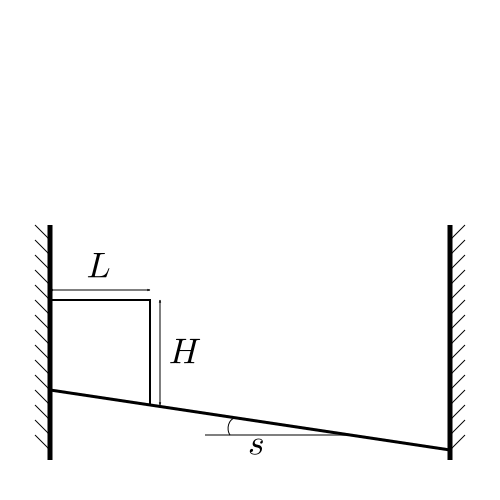
\includegraphics[width=0.4\textwidth,bb = 0 0 200 100, draft, type=eps]{/home/leo/Desktop/SVN/dassflow-2d/trunk/doc/figs/dambreak.svg}\caption{dam-break problem sketch.\label{fig:dambreak-sketch}}
\end{figure}
\par\end{center}

As no analytical solution can be derived, two converge simulations
are again performed with 12800 cells for $H=5\ m$ at time $t=500\ s$
and for $H=1\ m$ at time $t=2000\ s$. After the initial simulation
time, a rarefaction wave goes upstream and interacts with the left
wall boundary while a shock wave goes downstream, both modifing the
initial water column shape. After a sufficient simulation time, the
water column completly disappears and the new water shape exhibits
more mass and stronger gradients downstream. The dynamic wet/dry front
is robustly captured by well-balanced first- and second-order schemes
without any cut-off water depth $h_{\epsilon}$ , despite that the
well-balanced property is needless for this problem. We have verify
that the schemes are stricly positive and do not generate any negative
water depth.

\begin{center}
\begin{figure}[tbh]
\begin{centering}
\includegraphics[width=0.5\textwidth,bb = 0 0 200 100, draft, type=eps]{/home/leo/Desktop/SVN/dassflow-2d/trunk/doc/figs/dam_h_5_conv.pdf}\includegraphics[width=0.5\textwidth,bb = 0 0 200 100, draft, type=eps]{/home/leo/Desktop/SVN/dassflow-2d/trunk/doc/figs/dam_h_5.pdf}
\par\end{centering}
\centering{}\caption{Idealized dam break problem with $H=5\ m$. (left) rates of convergence
for the norm $e_{1}(h)$ for different schemes; (right) corresponding
initial condition, converge simulation with 12800 cells and results
with 100 cells.\label{fig:dam-break_h_5}}
\end{figure}
\par\end{center}

\begin{center}
\begin{figure}[tbh]
\centering{}\includegraphics[width=0.5\textwidth,bb = 0 0 200 100, draft, type=eps]{/home/leo/Desktop/SVN/dassflow-2d/trunk/doc/figs/dam_h_1_conv.pdf}\includegraphics[width=0.5\textwidth,bb = 0 0 200 100, draft, type=eps]{/home/leo/Desktop/SVN/dassflow-2d/trunk/doc/figs/dam_h_1.pdf}\caption{Idealized dam break problem with $H=1\ m$. (left) rates of convergence
for the norm $e_{1}(h)$ for different schemes; (right) corresponding
initial condition, converge simulation with 12800 cells and results
with 100 cells.\label{fig:dam-break_h_1}}
\end{figure}
\par\end{center}

Observing the relative error norms $e_{1}(h)$ in Fig.\ref{fig:dam-break_h_5}
and Fig.\ref{fig:dam-break_h_1}, on can first note that the previous
obtained second-order convergence rate is loosed due to the singularities
in the numerical solution and especially at wet/dry front. Nevertheless,
the relative error norm $e_{1}(h)$ is smaller for a given grid size
using the IMEX time stepping rather than the hybrid RK2 one and even
more comparatively to the first order schemes. If there is no major
difference between the schemes with or without the well-balanced property
when initially $H=5\ m$, this difference is obvious when $H=1\ m$.
The well-balanced second-order scheme with the hybrid RK2 time stepping
gives a result very similar to the first order scheme without the
well-balanced property. This indicates a drawback in both well-balanced
methods when the water depth is close to the bathymetry difference.
Sufficiently important to give very wrong numerical solutions with
first order schemes. In conclusion, in order to use these methods
to simulate hydraulic flows, one may be careful to verify this criteria
to produce meshes.

\subsection{simple channel}

In order to perform river flood simulations with real topography,
it is interesting now to check the numerical model behavior to simulate
an open-channel flow with a non constant topography gradient.

\subsubsection{Mac Donald's benchmark}

As it would be too restrictive to consider a channel with a constant
topography gradient, the Mac Donald's analytic steady solution for
open-channel flow is prefered \cite{MacDonald1997}. Making the hypothesis
of a contant discharge in space, it can be easily verify that the
steady states verify,

\begin{equation}
\begin{array}{c}
\partial_{t}h=\partial_{t}q=\partial_{x}q=0\\
\\
\partial_{x}z_{b}=\left({\displaystyle \frac{q^{2}}{gh^{3}}-1}\right)\partial_{x}h-{\displaystyle \frac{n^{2}q^{2}}{h^{10/3}}}
\end{array}\label{eq:open-channel-sol}
\end{equation}

that gives analytical steady solutions with a non necessary constant
topography gradient. We consider like in \cite{Delestre2012} a computational
domain lenght $l_{x}=1000\ m$, a lineic discharge $q=2\ m^{2}/s$
and a Manning-Strickler roughness coefficient $n=0.033$. Considering
this exact water depth,

\begin{equation}
h^{\text{exact}}(x)=\left({\displaystyle \frac{4}{g}}\right)^{1/3}\left(1+{\displaystyle \frac{1}{2}\exp\left(-16\left({\displaystyle \frac{x}{1000}-\frac{1}{2}}\right)^{2}\right)}\right)\label{eq:mcdonald_exact_h}
\end{equation}

insuring that the flow is subcritical in all the channel, the bottom
topography is numerically integrated with appropriate accurary that
gives the xyplot Fig.\ref{fig:mcdonald_sol}.

\begin{center}
\begin{figure}[tbh]
\centering{}\includegraphics[width=0.5\textwidth,bb = 0 0 200 100, draft, type=eps]{/home/leo/Desktop/SVN/dassflow-2d/trunk/doc/figs/channel_exact.pdf}\caption{Open-channel steady state solution (\ref{eq:open-channel-sol}) considering
the exact water depth (\ref{eq:mcdonald_exact_h}). \label{fig:mcdonald_sol}}
\end{figure}
\par\end{center}

The discharge is imposed upstream of the flow and the exact water
depth is prescribed downstream. Initialising the simulations with
dry cells except at the first cell at inflow, the steady states are
properly achieved in time. The relative error norms $e_{1}(h)$ and
$e_{1}(q)$ showed in Fig.\ref{fig:mcdonald_res} give the same result
than for the previous ``regularised'' dam break problem. The well-balanced
second order scheme with the hybrid RK2 time stepping is only first
order accurate with a smaller error than for the first order whereas
with the IMEX time stepping the numerical model is formally at second
order with very small errors even for very coarse meshes. A surprising
result is that this rate of convergence is obtained with non trivial
inflow/outflow boundary conditions even if this benchmark problem
is only onedimensional.

\begin{center}
\begin{figure}[tbh]
\centering{}\includegraphics[width=0.5\textwidth,bb = 0 0 200 100, draft, type=eps]{/home/leo/Desktop/SVN/dassflow-2d/trunk/doc/figs/channel_conv.pdf}\includegraphics[width=0.5\textwidth,bb = 0 0 200 100, draft, type=eps]{/home/leo/Desktop/SVN/dassflow-2d/trunk/doc/figs/channel_xy.pdf}\caption{Open-channel benchmark results : (left) relative error norms $e_{1}(h)$
and $e_{1}(q)$, $n$ is the cells number; (right) exact solutions
for $h$ and $u$ and simulations with 25 cells.\label{fig:mcdonald_res}}
\end{figure}
\par\end{center}

\subsubsection{perturbed topography}

The topography is not so smooth in real-life than in the previous
test case where a channel $1000\ m$ long was considered. It is tested
here the numerical model introducing gradually in frequency some perturbations
to an initial channel $10000\ m$ long with a constant slope of $0,25\ \%$
such that,\textcompwordmark{}

\begin{equation}
\begin{array}{c}
{\displaystyle z_{b}=z_{b}+\sum_{i=1}^{n_{p}}0.25\sin\left({\displaystyle 2\pi\left({\displaystyle \frac{p_{i}\ x}{l_{x}}}+r_{i}\right)}\right)}\quad\text{with}\quad r_{i}\in\left[0,1\right]\end{array}\label{eq:channel_perturb}
\end{equation}

with $n_{p}=1,2,3,4,5\ \text{and}\ 6$ and $p_{i}=7,24,57,108,205\ \text{and}\ 402$.
In order to control the flow at inflow and outflow, and especially
the backwater curve at the inflow, the topography gradient is kept
constant close to taking care to maintain perburtations spatially
continuous. The other parameters are a Manning-Strickler roughness
coefficient $n=0.05$, a lineic discharge $q=1\ m^{2}/s$ and a gravitational
acceleration $g=10\ m.s^{-1}$. Since the exact solution for the initial
constant slope channel is $h=1\ m$ (and $u=1\ m/s$), the topography
perturbations are of the same order of magnitude. The opposite case
would be obviously irrelevant. Main goal is to find a criteria that
insures a good accuracy to apply the numerical model with real topography.
Simulations are performed with the well-balanced second-order scheme
and the IMEX time stepping until the steady state is properly found.
For each of these six cases, a converge simulation is performed with
12800 cells of discretization showed at the left of the Fig.\ref{fig:channel_perturb_res}.
One can note that the flow respects the SW model hypothesis since
the smaller wavelength has a value of $25\ h$.

\begin{center}
\begin{figure}[tbh]
\centering{}\includegraphics[width=0.5\textwidth,bb = 0 0 200 100, draft, type=eps]{/home/leo/Desktop/SVN/dassflow-2d/trunk/doc/figs/perturb_bathy_channel_exact.pdf}\includegraphics[width=0.5\textwidth,bb = 0 0 200 100, draft, type=eps]{/home/leo/Desktop/SVN/dassflow-2d/trunk/doc/figs/perturb_bathy_channel_conv.pdf}\caption{Channel $10000\ m$ long with a constant slope of $0,25\ \%$ introducing
gradually in frequency some perturbations in topography according
to (\ref{eq:channel_perturb}) : (left) six cases with channel bottom
topography and associated converge simulations; (right) associated
relative error norm $e_{1}(h)$ with $n$ cells of discretization
(the greyer zone corresponds to less than 4 cells of discretization
for the highest frequency for each case).\label{fig:channel_perturb_res}}
\end{figure}
\par\end{center}

The calculation of the relative error norms $e_{1}(h)$ evolving the
mesh step size $n$ shows in Fig.\ref{fig:channel_perturb_res} that
introducing gradually in frequency some perturbations in the topography
damages the simulations accuracy. This phenomenom is in a first time
likely proportional to the highest perturbation frequency before saturing
when the mesh is too coarse comparatively to the highest frequency
introduced. The criteria to maintain a good accuracy as the right
correct second-order convergence rate is to discretize the channel
topography with a minimum of four points for the highest perturbation
frequency.

\subsection{Solitary wave on a simple beach}

It is well know that the SW equations can be a suitable model to study
numerically storm surges as the complete life-cycle of a tsunami (generation,
propagation and run-up on the coast). The classic benchmark problem
was introduced by Synolakis and al. \cite{Synolakis1987} deriving
an adimensionnal analytical solution for the run-up of a solitary
wave on a simple sloping beach. Following the parameters retained
in the NOAA technical report for evaluation of tsunami numerical models
\cite{Synolakis2007}, the initial condition with dimensional parameters
sketched in Fig.\ref{fig:beach_sketch} is,

\begin{equation}
\eta(x,0)=H\ sech^{^{2}}\left(\gamma\left({\displaystyle \frac{x-x_{0}-L}{d}}\right)\right)\quad\text{and}\quad u(x,0)=-\sqrt{{\displaystyle \frac{g}{d}}}\ \eta(x,0)
\end{equation}

with $\cot\beta=19.85$, $\gamma=\sqrt{3H/4d}$ and $L=\text{arccosh}\left(\sqrt{20}\right)/\gamma$.
The wave height satifies the adimendional parameter $H/d=0.0185$.
The computational domain is $100\:d$ long, the mesh step size respects
$\Delta x=d/10$ and wall boundaries conditions are prescribed. Using
the well-balanced second-order numerical scheme with the MP limter
and IMEX time stepping, resulting water levels profiles and two time
series are plotted in Fig.\ref{fig:beach_res} as superposed the nonlinear
analytical solution.

\begin{center}
\begin{figure}[tbh]
\begin{centering}
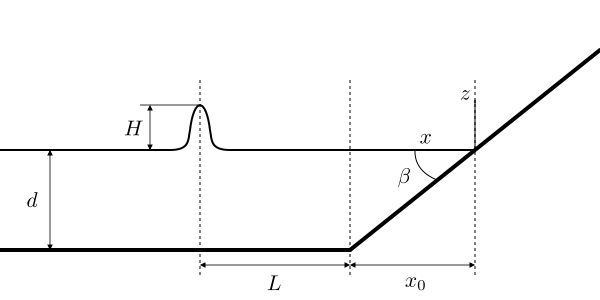
\includegraphics[width=0.5\textwidth,bb = 0 0 200 100, draft, type=eps]{/home/leo/Desktop/SVN/dassflow-2d/trunk/doc/figs/plane_beach.svg}
\par\end{centering}
\centering{}\caption{Dimensional sketch of the solitiary wave run-up benchmark problem
sketch.\label{fig:beach_sketch}}
\end{figure}
\par\end{center}

\begin{center}
\begin{figure}[tbh]
\centering{}\includegraphics[width=0.5\textwidth,bb = 0 0 200 100, draft, type=eps]{/home/leo/Desktop/SVN/dassflow-2d/trunk/doc/figs/beach_t_35_45_55_65.pdf}\includegraphics[width=0.5\textwidth,bb = 0 0 200 100, draft, type=eps]{/home/leo/Desktop/SVN/dassflow-2d/trunk/doc/figs/beach_x_0.25_9.95.pdf}\caption{Run-up of a solitiary wave on a simple beach : comparison of analytical
solution (scatters) versus numerical solution (solid lines).\label{fig:beach_res}}
\end{figure}
\par\end{center}

According to Synolakis and al. in \cite{Synolakis2007} page 5, \textquotedblleft \textit{any
well benchmarked code should produce results within 5\% of the calculated
value from the analytical solution}'' which is the case for our simulation
which is spatially everywhere very close to the analytical solution.
There is no particular ``distortion'' in the numerical solution
at adimensional time $t/\tau=45\ \text{and}\ 65$ in proximity to
the wet/dry front whereas other numerical models can produce some
like it is showed in the NTHMP workshop report \cite{2012}. This
demonstrates that our well-balanced treatment at wet/dry front do
not affect a wave run-up computation accuracy.

\bibliographystyle{plain}
\bibliography{references}

\end{document}
